\section{Capico}

Suite à la formation et au mini-projet d'e-banking, j'ai intégré l'équipe travaillant sur le projet Capico. Je vais donc commencer par expliquer le projet puis détailler le travail effectué sur ce projet.

\subsection{Historique}

Capico a été à l’origine développé pour une utilisation en interne, pour laquelle il n’était attendu que peu de connexions simultanées. Le projet a évolué au fil du temps, grandissant tant en terme de fonctionnalités qu’en terme de technologies. On a ainsi pu passer d’OpenLaszlo à Flex pour obtenir une RIA (Rich Internet Application).\\

Aujourd’hui, eBusiness Information souhaite tout de même étendre l’utilisation de Capico, notamment pour l’Éducation Nationale. Mais cette application n’ayant jamais eu avant l’année dernière de réel architecte logiciel pour suivre correctement son évolution, aucune réelle étude de volumétrie n’a à ce jour été effectuée pour s’assurer que l’application puisse soutenir la charge requise.\\

À la rentrée de septembre, l’Académie de Créteil va être amenée à utiliser le logiciel Capico pendant une période de test, et c’est ainsi que 5000 nouveaux utilisateurs vont devoir accéder à cette application, avec globalement une moyenne de 20 connexions simultanées sur la plateforme Capico.\\

L'objectif pour le projet Capico est donc de préparer l'application pour une mise en production avec un nombre importants d'utilisateurs. Ce qui implique de tester l'application de fond en comble, corriger les bugs découverts, effectuer des tests de charges et rendre l'application plus robuste.

\subsection{Fonctionnalités}

La formation initiale nous a permis d’utiliser les fonctionnalités de base de Capico : la lecture de cours, la réponse à des QCMs et à des exercices. Néanmoins, cela correspond à la seule vue d’un élève de Capico. Il y a globalement trois niveaux d’accès à l’application : élève, professeur, et administrateur. Chaque rôle vient avec son lot de fonctionnalités plus ou moins limitées.\\

\begin{description}
	\item[Les élèves] peuvent :
	\begin{itemize}
		\item consulter des cours mis à leur disposition dans leur bibliothèque,
		\item répondre à des QCMs (figure \ref{fig:qcm}),
		\item effectuer le travail demandé dans l'onglet \flqq{}travail à faire\frqq{},
		\item ajouter, chatter ou partager leur bureau avec des contacts,
		\item poster des commentaires.
	\end{itemize}
	
	\item[Les professeurs] peuvent :
	\begin{itemize}
		\item effectuer toutes les actions disponibles aux élèves,
		\item créer de nouveaux contenus (cours, dossiers, exercices, \dots{}) depuis leur onglet \flqq{}bureau\frqq{} (figure \ref{fig:creation_contenu}),
		\item sonoriser des contenus (figure \ref{fig:sonorisation}),
		\item créer et administrer des classes d'élèves,
		\item suivre l'évolution d'élèves, leur donner du travail à faire.
	\end{itemize}
	
	\item[Les administrateurs] peuvent :
	\begin{itemize}
		\item effectuer toutes les actions disponibles aux professeurs,
		\item éditer et visualiser l'ensemble des contenus présents sur la plateforme \capico{} (figure \ref{fig:administration}).
	\end{itemize}
\end{description}

\begin{figure}[H]
	\centering
	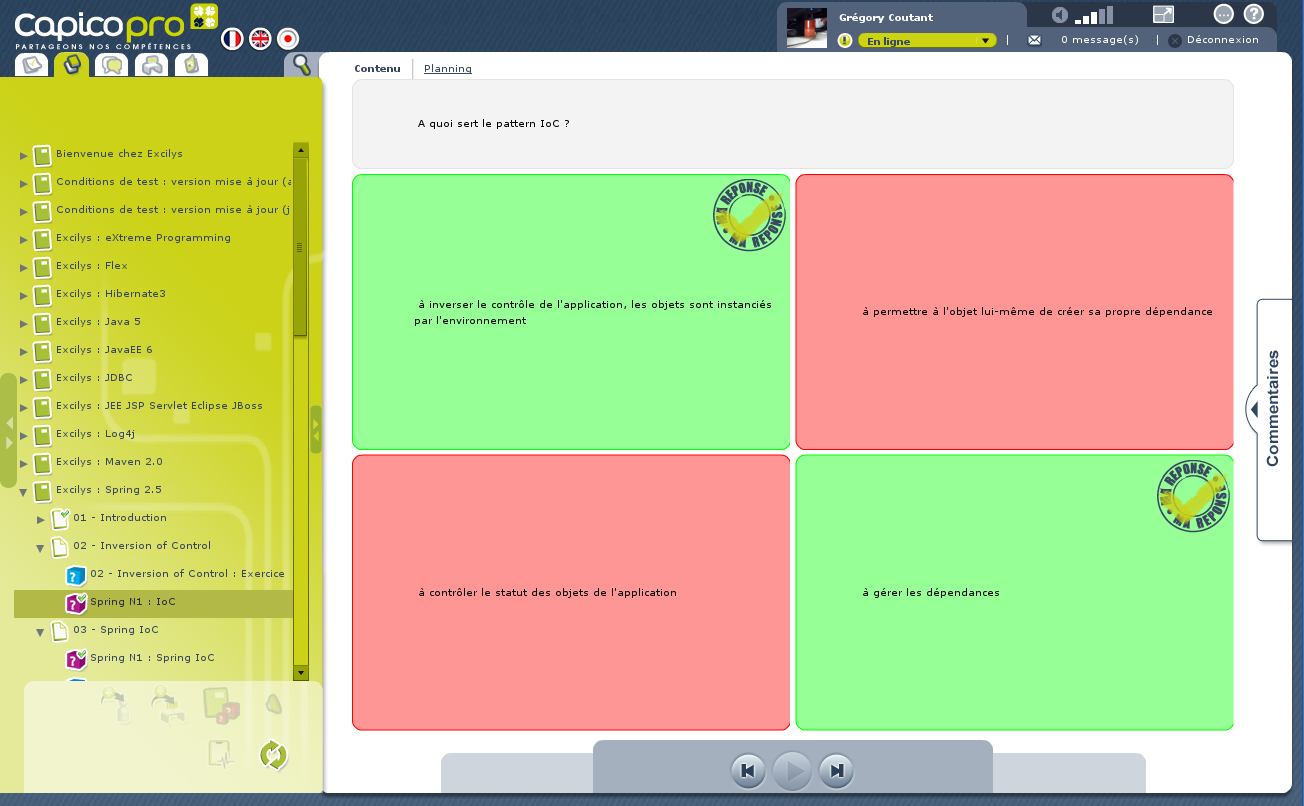
\includegraphics[width=\textwidth]{images/qcm.pdf}
	\caption{Interface d'un questionnaire dans \capico{}}
	\label{fig:qcm}
\end{figure}

\begin{figure}[H]
	\centering
	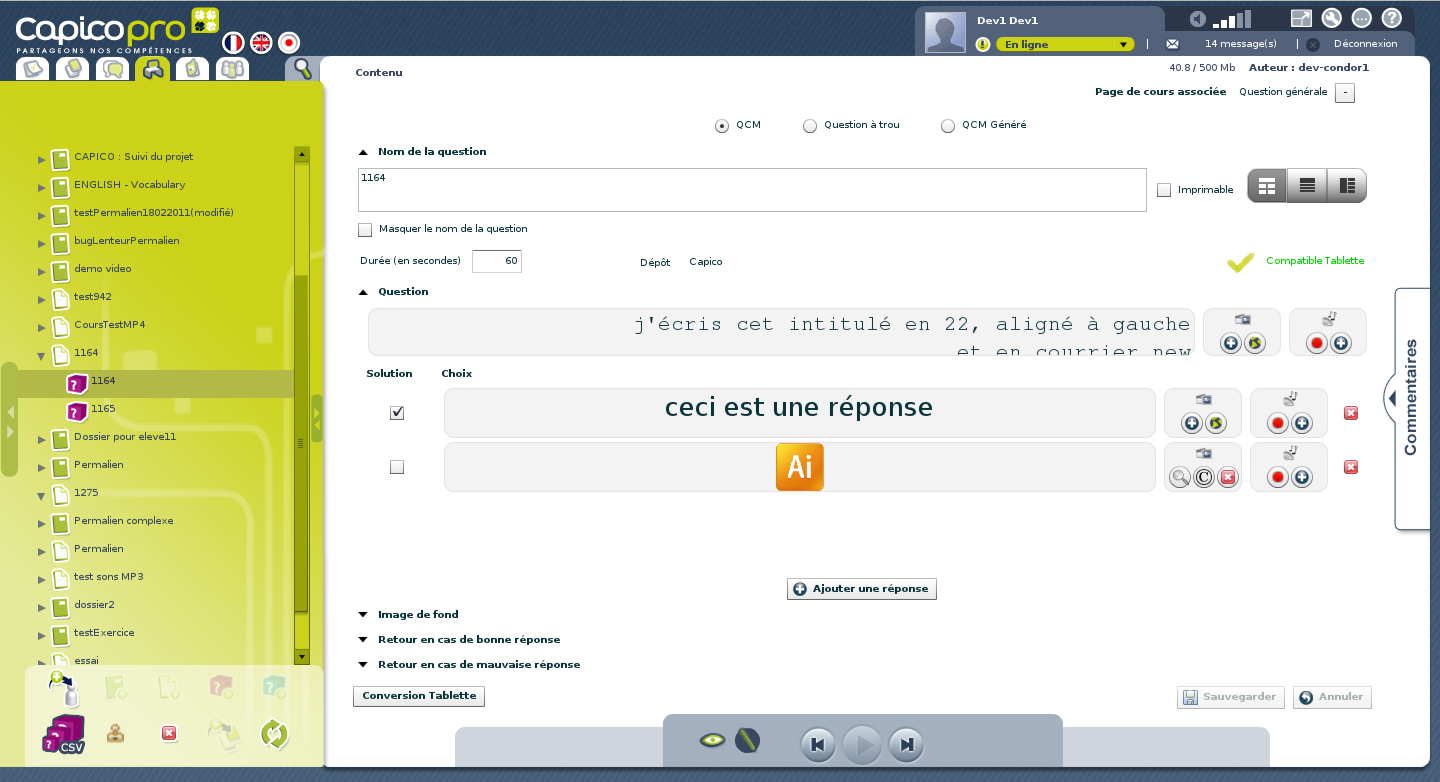
\includegraphics[width=\textwidth]{images/creation_contenu.pdf}
	\caption{Interface de création de questions}
	\label{fig:creation_contenu}
\end{figure}

\begin{figure}[H]
	\centering
	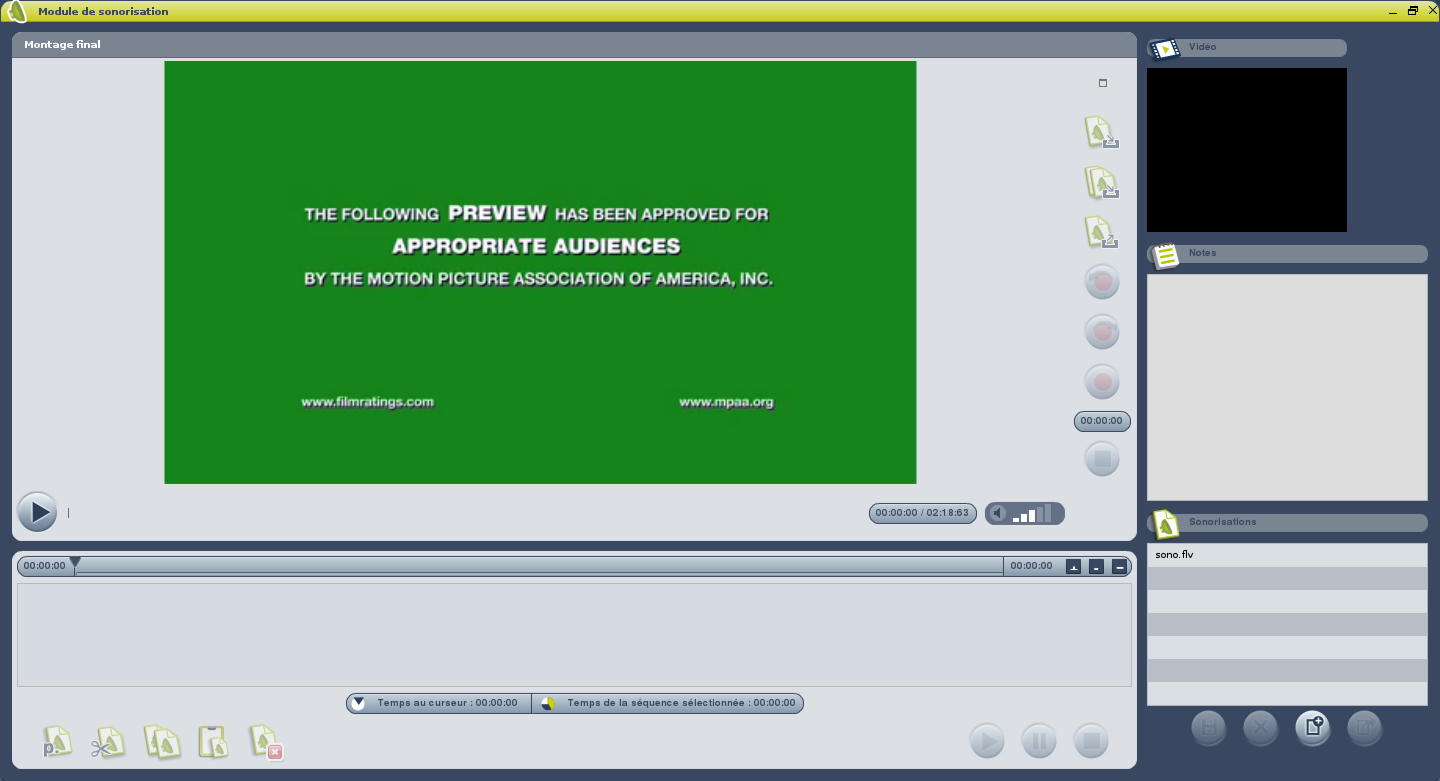
\includegraphics[width=\textwidth]{images/sonorisation.pdf}
	\caption{Interface de sonorisation de cours}
	\label{fig:sonorisation}
\end{figure}

\begin{figure}[H]
	\centering
	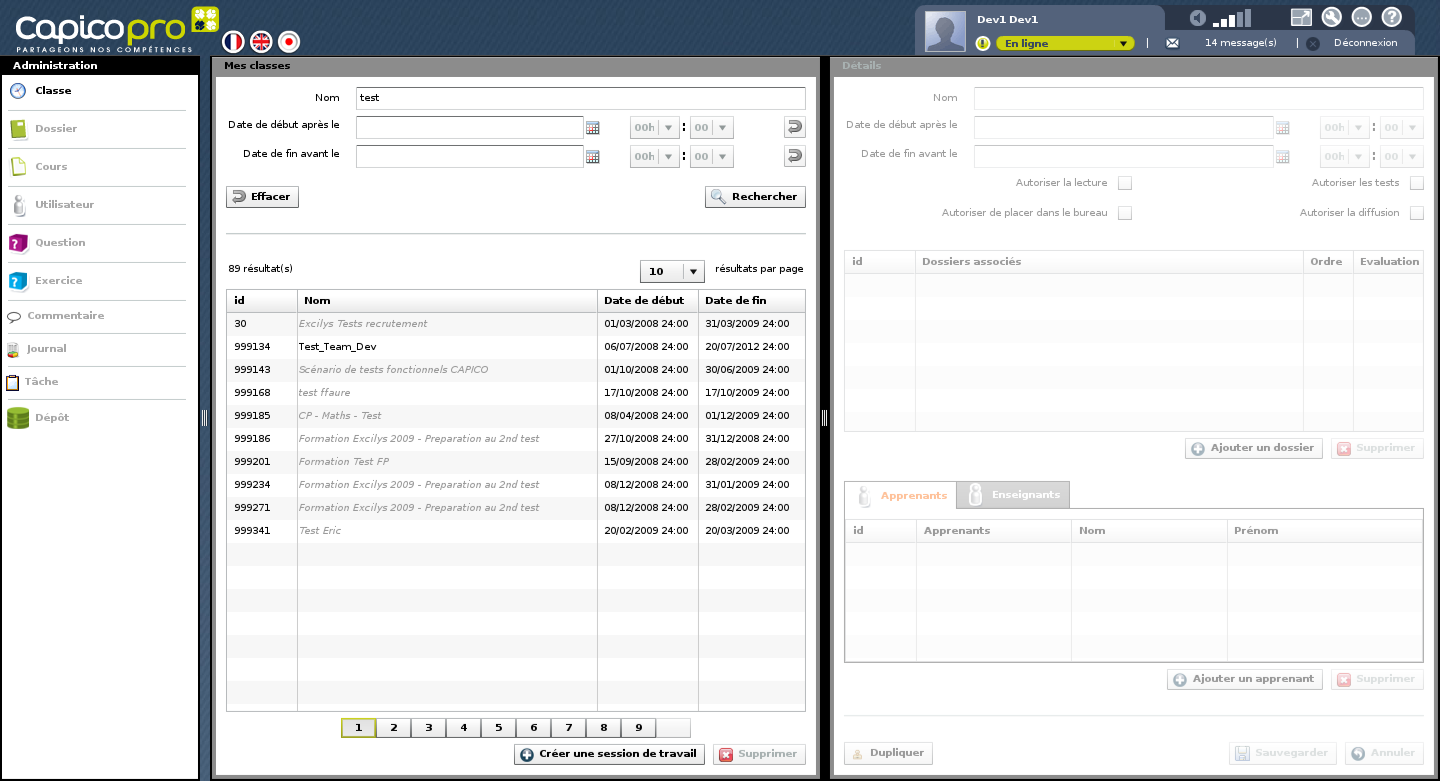
\includegraphics[width=\textwidth]{images/administration.png}
	\caption{Interface d'administration de \capico{}}
	\label{fig:administration}
\end{figure}

L'ensemble des fonctionnalités de Capico est présentée de manière plus abrupte dans la figure suivante :

\begin{figure}[H]
	\centering
	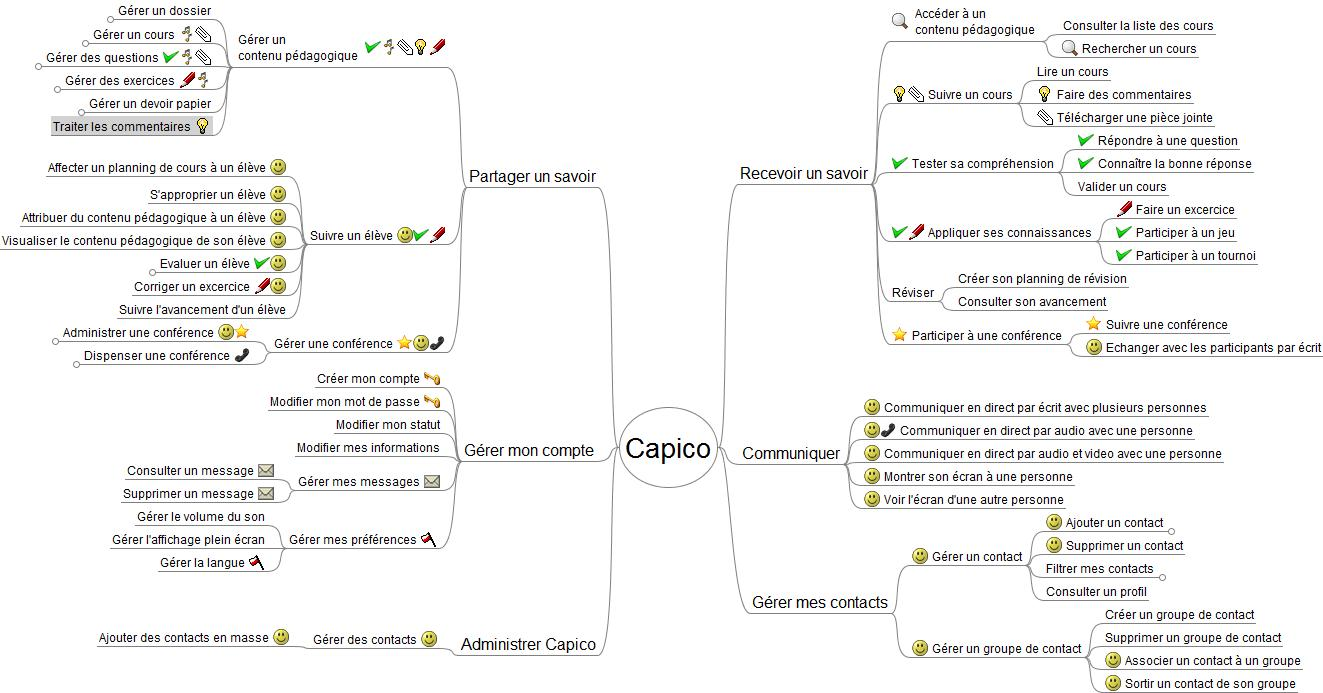
\includegraphics[width=\textwidth]{images/capico_carto_fonctionnelle.pdf}
	\caption{Cartographie fonctionnelle de \capico{}}
\end{figure}

\subsection{Architecture}

L'architecture globale de l'application est présentée ci-après :

\begin{figure}[H]
	\centering
	\includegraphics[width=0.8\textwidth]{images/architecture_capico.pdf}
	\caption{Architecture globale de \capico{}}
\end{figure}

Globalement, le projet est subdivisé en deux parties majeures développées par \excilys{} dans des technologies différentes. La première partie, appelée \flqq{}front-end\frqq{}, est développée en Flex et constitue l'interface avec l'utilisateur final. La seconde partie est le \flqq{}back-end\frqq{}, développé globalement en Java et qui présente la logique métier accessible au front-end. Une dernière partie à part et non développée ici est la partie SecuAdmin qui gère les droits des différents utilisateurs.\\

Les projets externes nécessaires au bon fonctionnement de \capico{} sont les suivants :

\begin{description}
	\item[Red5] est le serveur permettant le streaming audio/vidéo dans Flash,
	\item[OpenFire] est le serveur de messagerie instantanée de \capico{}, basé sur le protocole XMPP,
	\item[MySQL] est le SGBD utilisé par \capico{} pour sauvegarder tous les contenus,
	\item[Alfresco] est un système de gestion de contenu qui stocke les fichiers (images, sons, vidéos, \dots{}) utilisés dans \capico{},
	\item[CAS] est le système d'authentification de \capico{},
	\item[LDAP] est l'annuaire contenant les informations sur l'ensemble des utilisateurs.\\
\end{description}

Voici maintenant la description détaillée du back-end et du front-end de \capico{}.

\subsubsection{Front-End}

Le front-end est séparé en deux projets principaux :

\begin{description}
	\item[capico-thick-front-end] qui contient les sources effectives de \capico{}
	\item[capico-front-player] chargé de fournir du contenu créé sur \capico{} par le biais d'un permalien.
\end{description}

À côté de ces deux projets se trouvent également un ensemble de sous-projets de librairies nécessaires à leur bon fonctionnement.\\

Concernant son architecture à proprement parler, le front-end repose sur le pattern MVC, auparavant à l'aide du framework Cairngorn, mais désormais sans framework particulier. L'implémentation tend maintenant à utiliser l'architecture présentée dans la figure suivante, qui utilise un \emph{manager} pour référencer les vues et transmettre les données du modèle nécessaires à celles-ci.

\begin{figure}[H]
	\centering
	\includegraphics[width=0.6\textwidth]{images/manager.pdf}
	\caption{Architecture du front-end}
\end{figure}


\subsubsection{Back-end}

Le back-end, en Java, suit une architecture en couche, sensiblement la même que celle réalisée pour l'application d'e-banking. Nous avons ainsi :

\begin{description}
	\item[Une couche d'entités] qui correspondent aux éléments utilisables partout dans notre application,
	\item[Une couche de DTO]  (Domain Transfer Object) qui représente les objets qui seront échangés entre le front-end et le back-end. Ceux-ci sont généralement des représentations simplifiées des objets du domaine, et qui permettent entre autres d'alléger la taille des messages échangés,
	\item[Une couche persistance] qui en utilisant Hibernate et le pattern DAO permet de persister nos données,
	\item[Une couche métier] qui contient, comme son nom l'indique, la véritable logique métier de l'application,
	\item[Une couche service] qui présente au front-end l'ensemble des méthodes qui lui sont accessibles.
\end{description}

\subsection{Appropriation}

L'ensemble de la plateforme \capico{} formant une application somme toute assez volumineuse (plusieurs milliers de lignes de code), il n'était pas possible de rentrer directement dans le code pour corriger des bugs ou implémenter de nouvelles fonctionnalités.\\

Afin de nous approprier la plateforme, notre équipe a donc, dans un premier temps, réalisé la recette de la version en pré-production du produit. Cela nous a ainsi permis de toucher à peu près à toutes les fonctionnalités de l'application, d'un point de vue utilisateur élève, professeur et administrateur.\\

Les erreurs repérées par notre équipe étaient ensuite répertoriées à l'aide d'un bug tracker dédié au projet, utilisant la plateforme Mantis. Celui-ci permet d'observer de manière simple les erreurs sur les diverses versions du produit, de les assigner à des correcteurs, et bien entendu de les clôturer une fois traitées.

\begin{figure}[H]
	\centering
	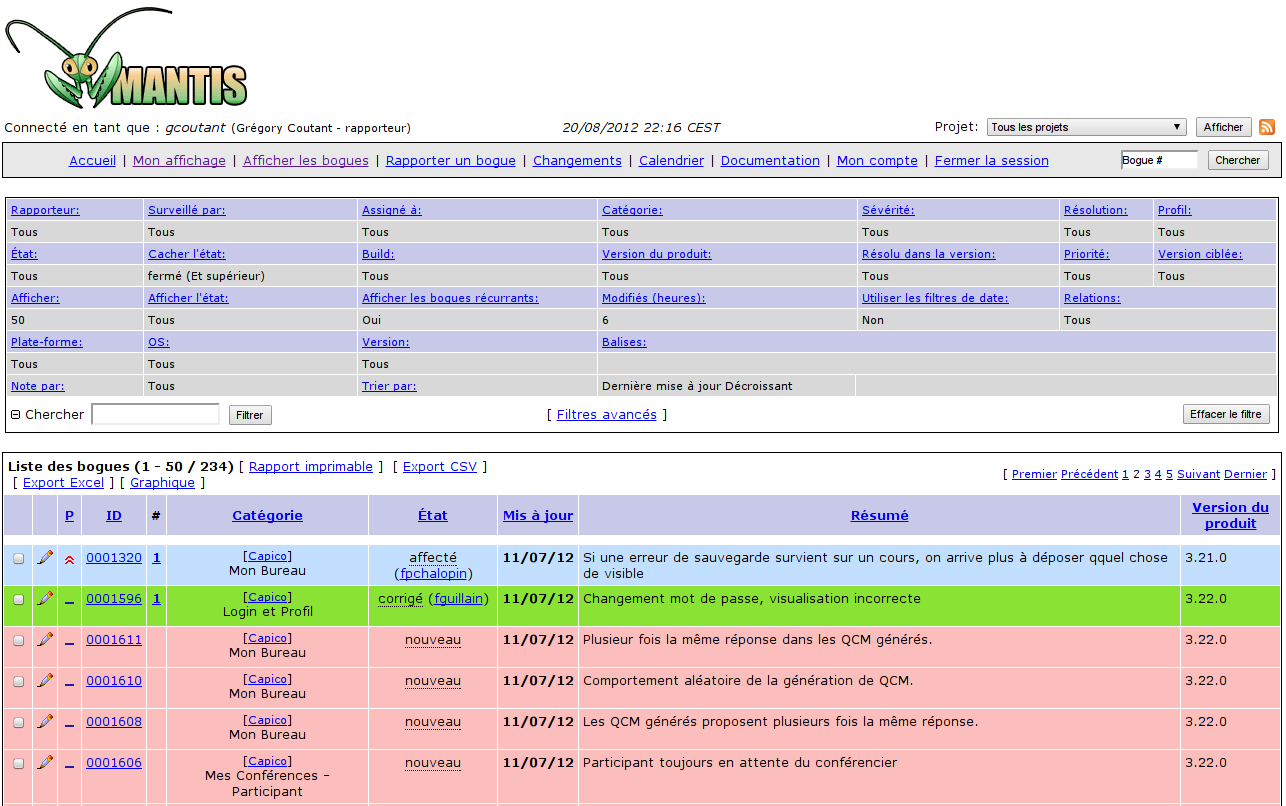
\includegraphics[width=\textwidth]{images/mantis.pdf}
	\caption{Outil de bug tracking}
\end{figure}

\subsection{Correction des bugs}

Une fois le fonctionnement de l'application assimilé, et afin de rentrer \flqq{}doucement\frqq{} dans le code, le responsable du projet nous a assigné, parmi les bugs que nous avions reporté, ceux qu'il estimait à notre portée. Nous avons ainsi pu nous faire la main sur du code à la fois Flex pour le front-end et Java pour les parties nécessitant des corrections sur le back-end (plus rare).\\

Pour cela, nous avons tout de même du mettre en place une machine virtuelle pour chacun de nos postes permettant de lancer un serveur faisant tourner l'application \capico{} en local prenant en compte nos modifications.

\subsection{Retour sur le projet Capico}

Bien que je ne sois pas resté très longtemps sur ce projet qu'est Capico (3 semaines), cette expérience aura été très enrichissante puisqu'il m'a permis de me rendre compte quelles pouvaient être les difficultés rencontrées lorsqu'on arrive sur un gros projet tel que celui-ci.\\

Je me suis retrouvé ainsi face à des fonctionnalités dont je n'avais aucune idée du fonctionnement mais qui présentaient des bugs qu'il fallait corriger. Je me suis donc renseigner sur les implémentations de ces fonctionnalités auprès des personnes qui connaissent son fonctionnement. J'ai bien évidemment explorer le code pour essayer de mieux en comprendre le fonctionnement. Le tout pour pouvoir finalement corriger le bug et avoir une meilleure compréhension de l'application.